%!TEX root = ../../../main.tex

\subsection{2D CNN based clip-level feature extraction}
    First, the ResNet-50 Convolution Neural Network \cite{he2016deep} is used as a 2D CNN network to extract spatial features of each frame in video. Fig.\ref{fig:resnet50} illustrates the architecture of ResNet-50 which composes of five convolutional blocks stacked on top of each other. The network is pre-trained on ImageNet then fine-tuned using training sets described in Section \ref{sec:experimentalresult}. Deep residual features are extracted from the output of the last convolutional block of the network which is a 2048-D feature vector. 
    \begin{figure}[htbp]
        \centering
        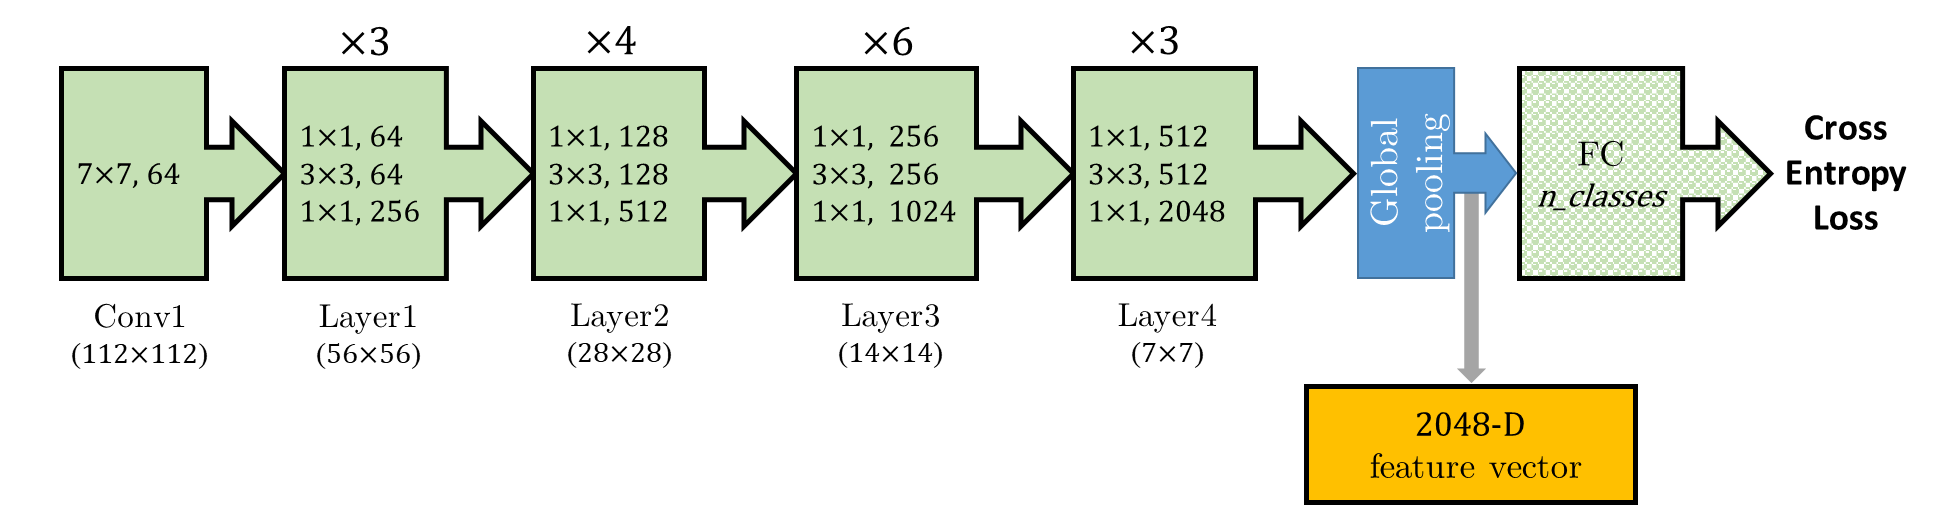
\includegraphics[width=1\linewidth]{Figs/Resnet50.png}
        \caption{Architecture of ResNet-50 utilized in our work for feature extraction at each separated view}
        %\vspace{-0.3cm}
        \label{fig:resnet50}
    \end{figure}
    We then aggregate frame-level features to create video-level features. In this work, we implement three temporal modeling techniques: 1) average pooling (AP); 2) recurrent neural network (RNN) and 3) temporal attention (TA). Fig.\ref{fig:pooling} illustrates three techniques.
    \begin{figure}[htbp]
        \centering
        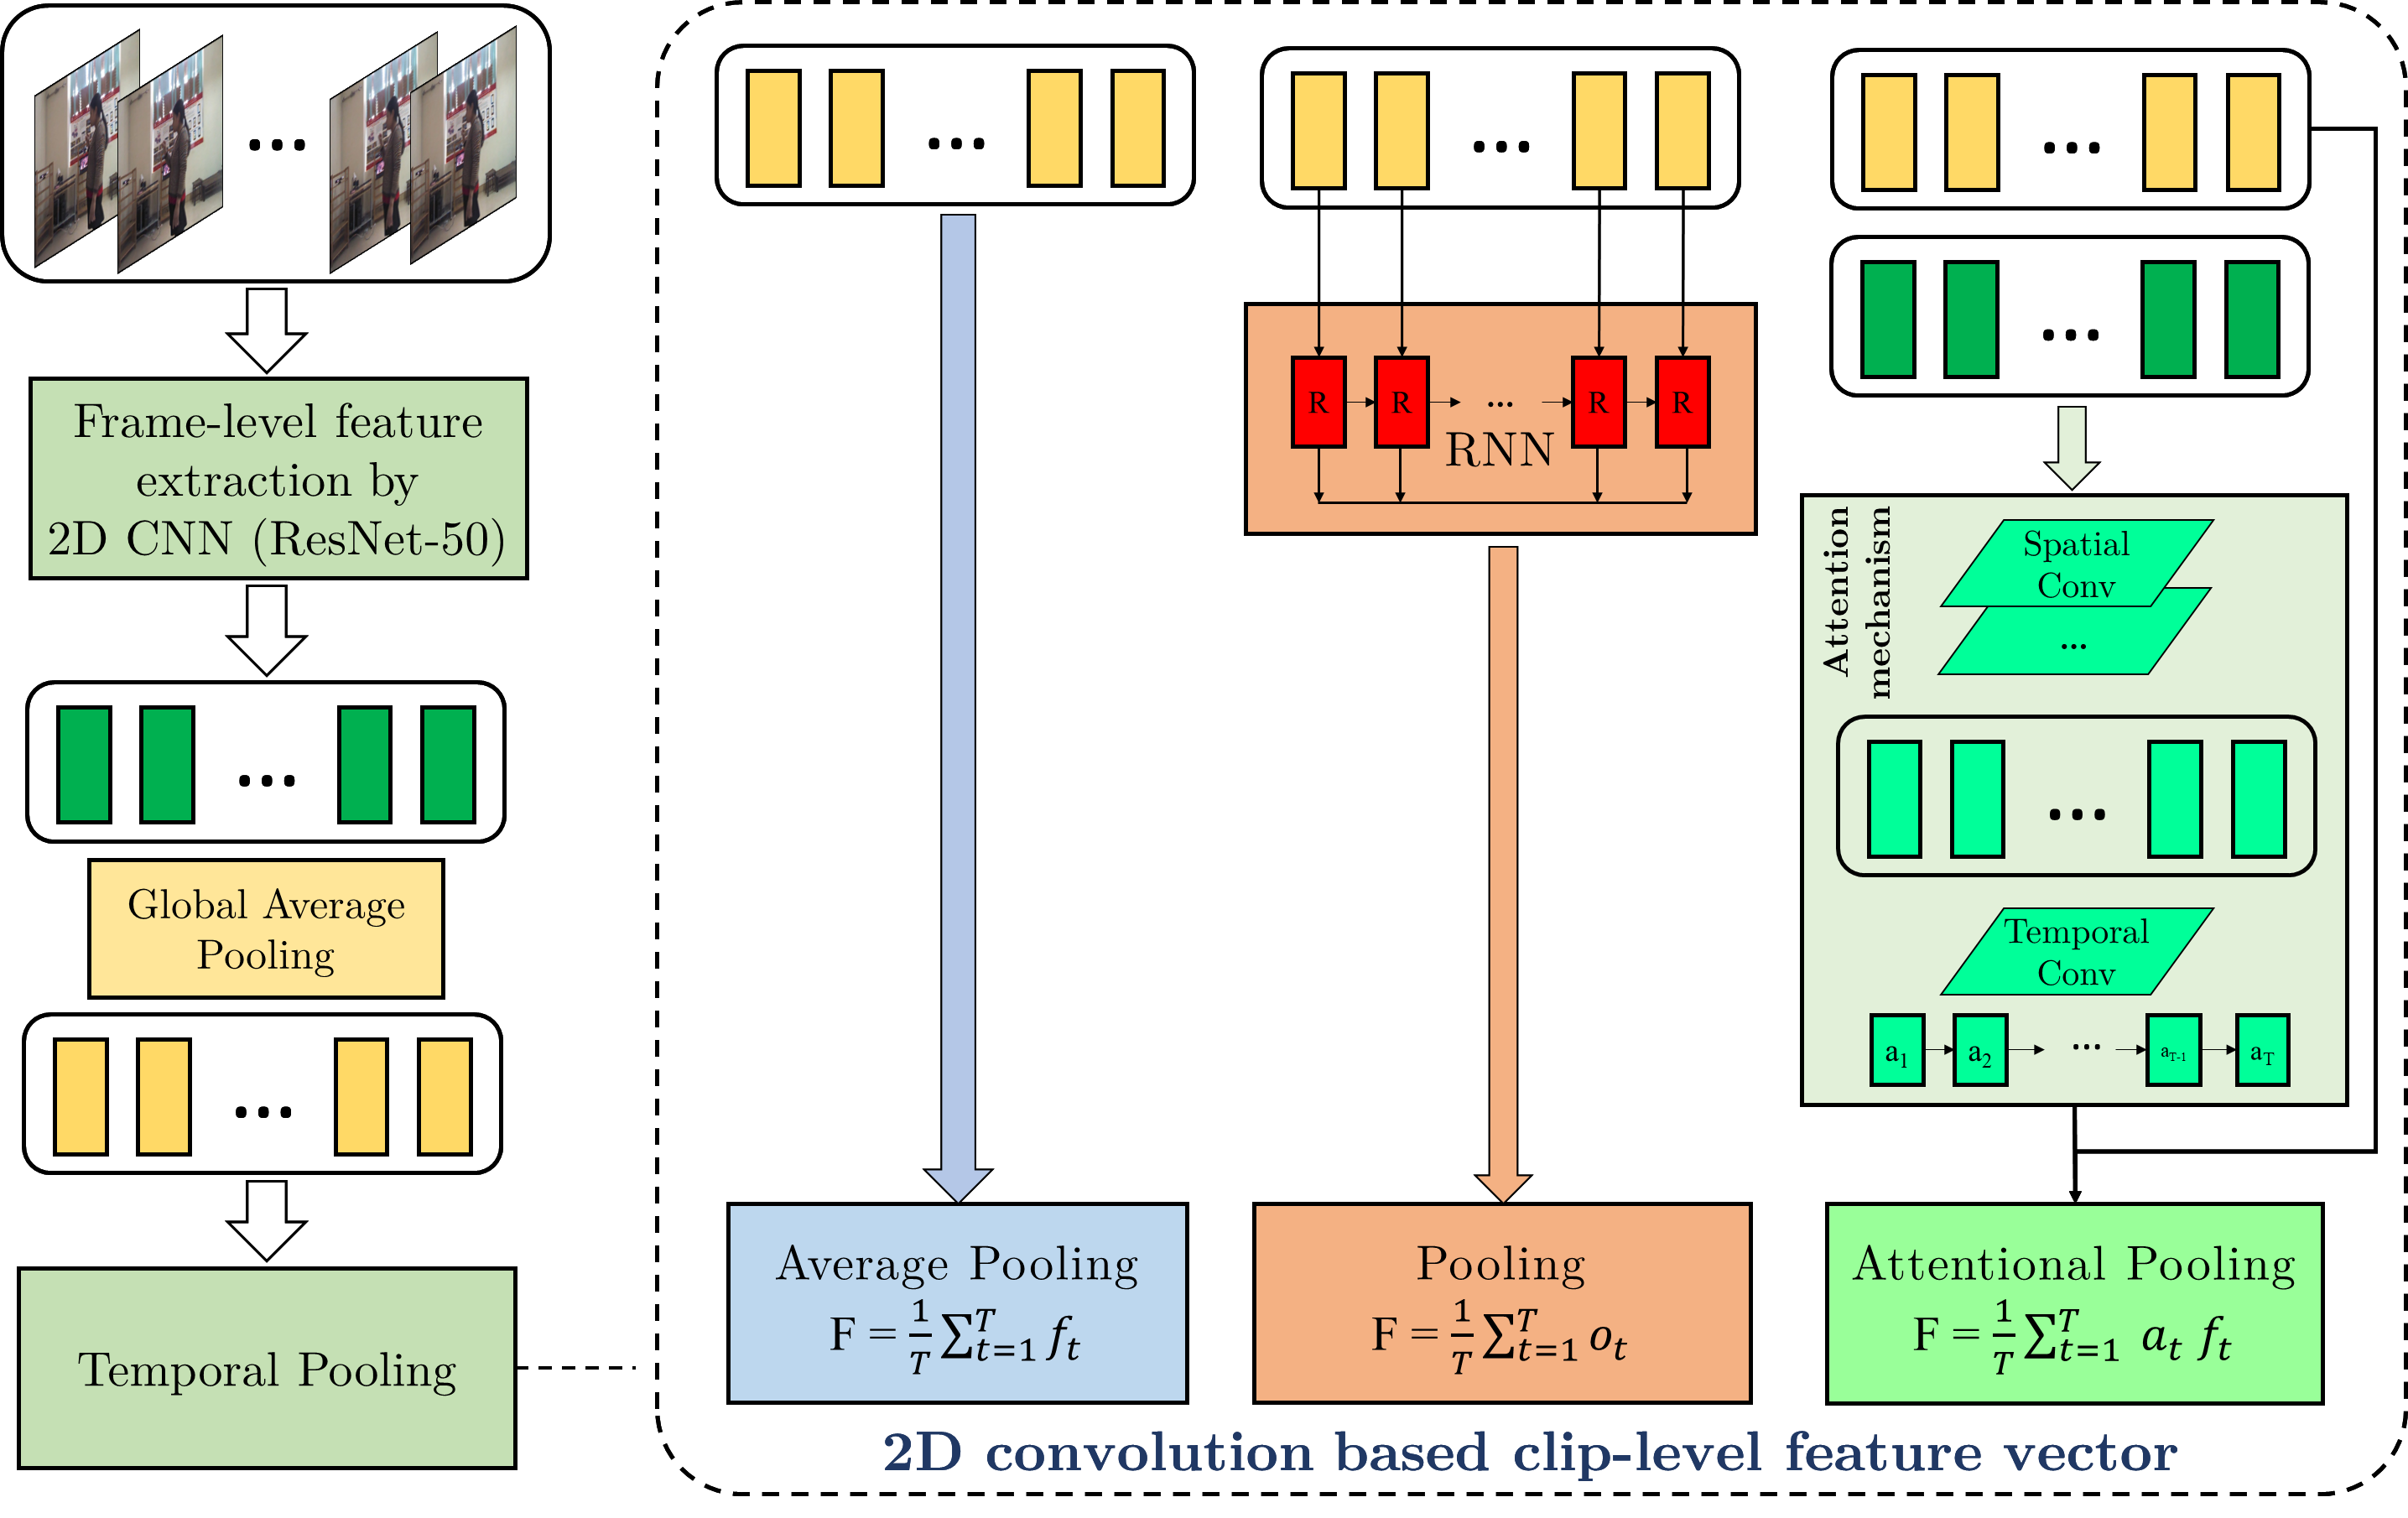
\includegraphics[width=1\linewidth]{Figs/Pooling.png}
        \caption{Three pooling techniques: Average Pooling (AP), Recurrent Neural Network (RNN) and Temporal Attention Pooling (TA)}
        %\vspace{-0.3cm}
        \label{fig:pooling}
    \end{figure}

    \textbf{Average Pooling - AP}: Let ${f}$ be the video-level feature, ${f_t}$ be the frame-level feature at time ${t}$, $T$ be the number of frames in video. Average pooling technique simply averages all frame-level features uniformly to create the video-level feature:
    \begin{equation}
    f=\frac{1}{T}\sum_{t=1}^T{f_t}
    \end{equation}
    As a frame-level feature is a 2048-D vector, the video-level feature is of the same dimension.\\
    \textbf{Recurrent Neural Network - RNN}: An RNN cell encodes a $t^{th}$ frame-level feature at time $t$ of the sequence and passes the hidden state $h_t$ into the next time step. In our work, a cell is a LSTM (Long Short Term Memory). The RNN is a single-layer with $T$ cells. Each cell outputs a 512-D feature vector that contains information of the current frame and the previous ones. We aggregate a sequence of frame-level features into a video-level feature $f$ by calculating the average of the RNN outputs $o_t = R(f_t, o_{t-1})$;$t \in [1;T]$. 
    \begin{equation}
    f=\frac{1}{T}\sum_{t=1}^T{o_t}
    \end{equation}
    \textbf{Temporal Attention - TA}: In the above pooling techniques, frame-level features are equally aggregated. In reality, some frames may have more important roles than remaining ones in recognizing an action. In temporal attention model, we learn a weight $a_t$ for each frame $f_t$ and apply an attention weighted average on the sequence of frame-level features as follows.
    \begin{equation}
    f=\frac{1}{T} \sum_{t=1}^{T}a_{t}f_{t}
    \end{equation}
    To learn the weights $a_t, t \in [1,T]$, we adopt the attention generation network proposed by Jiyang Gao et al. \cite{gao2018revisiting}. The network takes a sequence of frame-level features $[T, w, h, 2048]$, each is tensor extracted from the last convolution layer of ResNet-50. The network architecture consists of two main components: Spatial Convolution and Temporal Convolution. First, a conv layer with shape $\{w,h,2048,d_t\}$ is applied, then we get a $d_t$-dimensional feature for each frame of the clip ($d_t$ = input channel). Then we apply a temporal conv layer $\{3,d_t, 1\}$ on these frame-level features to generate temporal attentions $s_c^t$. Once we have $s_c^t$, the final attention score $a_t$ is computed by Softmax function: 
    \begin{equation}
    a_t = \frac{e^{s_c^t}}{\sum_{k=1}^{T}e^{s_c^k}}
    \end{equation}
    %In all scenarios of pooling, we train the whole net (including a ResNet-50 combined with RNN, TA or AP) on our training set according to the evaluation protocols presented in section \ref{sec:experimentalresult}.
